\chapter{Introdução}

\section{Seção 1 do Capítulo 1}
\subsection{Subseção}
\subsubsection{Subsubseção}

A Figura \ref{fig:sistemaProposto}. A Tabela \ref{tab:tabelaTeste}. A Equação (\ref{eq1}). O trabalho de fulano~\cite{ref1}. O Código Fonte \ref{cod1}.

\begin{figure}[htbp]	
\begin{center}
		\fbox{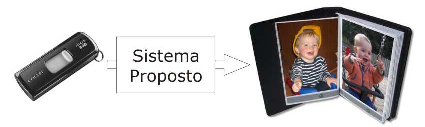
\includegraphics[scale=1]{figs/sistemaProposto.pdf}}
	\end{center}
	\caption{Sistema proposto}
	\label{fig:sistemaProposto}
\end{figure}

\begin{table}[htpb]
\begin{center}
\begin{tabular}{|c|c|c|}
\hline
coluna 1 & coluna 2 & coluna 3 \\
\hline
valor 1,1 & valor 1,2 & valor 1,3 \\
valor 2,1 & valor 2,2 & valor 2,3 \\
\hline
\end{tabular}
\end{center}
\caption{Primeira tabela.}
\label{tab:tabelaTeste}
\end{table}

\begin{equation}
E = m \times c^2
\label{eq1}
\end{equation}

\begin{lstlisting}[caption={Loop simples},label=cod1,numbers=none]
for(int x=1; x<10; x++){
  cout << x << "\n";
}
\end{lstlisting}

\section{Seção 2 do Capítulo 1}
\subsection{Subseção}
\subsubsection{Subsubseção}

